% =========================================================================
% STC-LoRA -- ICLR-style submission draft
% Self-contained preamble approximating the ICLR template. At submission,
% replace the FALLBACK PREAMBLE block with:
%     \usepackage{iclr20XX_conference,times}
% from the official template and delete the geometry/titling lines.
% Build:  latexmk -pdf main.tex
% =========================================================================
\documentclass{article}

% ---------- FALLBACK PREAMBLE (approximates ICLR layout) ----------------
\usepackage[letterpaper,margin=1in]{geometry}
\usepackage{times}
\usepackage[numbers,sort&compress]{natbib}
\setlength{\parskip}{2pt}
% -------------------------------------------------------------------------

\usepackage{amsmath,amssymb,bm}
\usepackage{booktabs}
\usepackage{graphicx}
\usepackage{xcolor}
\usepackage[colorlinks=true,linkcolor=blue,citecolor=blue,urlcolor=blue]{hyperref}

\newcommand{\stc}{STC-LoRA}
\newcommand{\best}[1]{\bm{#1}}   % bold in math mode (used inside $...$)

\title{Synaptic Tagging and Capture for Continual Learning\\in Frozen Language Models}
\author{Kit Fung, Chai\\Cortexum\\\texttt{kit@cortexum.ai}}
\date{}

\begin{document}
\maketitle

\begin{abstract}
Deployed language models cannot absorb new information without retraining, and naive fine-tuning induces catastrophic forgetting. We introduce \stc{}, a parameter-efficient continual-learning adapter for a \emph{frozen} pretrained LM, motivated by the neuroscience of synaptic tagging and capture: each adapted weight carries a fast, \emph{decaying} low-rank delta updated on every exposure, and a \emph{permanent} store that grows only when a surprise-derived gate fires, consolidating transient changes into durable memory. On a boundary-free, online, domain-incremental benchmark, \stc{} reduces backward-transfer forgetting from $+39.2\%$ (naive LoRA) to $+3.8$--$5.4\%$ at 0.5B parameters, and the advantage strengthens with scale --- error-barred at 0.5B, 1.5B, and 7B: at 7B, naive fine-tuning still forgets $+20.2\%$ and Experience Replay $+14.7\%$, while \stc{} forgets ${\approx}0\%$ with ${\approx}5\times$ lower variance across task orderings. The ordering reproduces exactly on a second model family (Llama-3.2-1B). Protection extends beyond perplexity: on downstream metrics (next-token accuracy, zero-shot news classification) \stc{} loses $5\times$ less capability than naive fine-tuning. A capacity-matched control shows the gain is mechanistic rather than a parameter artifact, and a matched non-adaptive ablation shows the surprise gate buys superior plasticity \emph{allocation}. The core variants require no rehearsal buffer of past data.
\end{abstract}

\section{Introduction}
A frozen pretrained language model is a fixed function: it cannot learn from deployment experience, and any online gradient update risks overwriting prior knowledge --- catastrophic forgetting \citep{mccloskey1989catastrophic}. Standard continual-learning (CL) remedies trade off along familiar axes: regularization constrains plasticity \citep{kirkpatrick2017overcoming,zenke2017continual}, and rehearsal stores past data \citep{rolnick2019experience}, raising storage and privacy costs.

Biological synapses face the same stability--plasticity dilemma and resolve it with \emph{synaptic tagging and capture} (STC) \citep{frey1997synaptic}: activity transiently \emph{tags} a synapse, but the change becomes persistent only if a neuromodulatory consolidation signal arrives while the tag is present; otherwise it decays. Complementary learning systems theory \citep{mcclelland1995there} likewise separates fast, labile acquisition from slow, durable consolidation. We treat this two-timescale, significance-gated design purely as an \emph{architectural motivation} and evaluate the resulting method on standard CL grounds.

We map STC onto low-rank adaptation \citep{hu2022lora} of a frozen transformer. Our contributions:
\begin{enumerate}
  \item \textbf{\stc{}} (\S\ref{sec:method}): a two-timescale LoRA adapter --- a decaying \emph{tagged} pair plus a slowly-plastic \emph{permanent} store --- with plasticity and consolidation gated by a surprise signal derived from the model's own loss. The core variants are rehearsal-free.
  \item \textbf{A boundary-free online benchmark and controlled comparison} (\S\ref{sec:setup}): naive LoRA, online EWC, Experience Replay, and A-GEM on a shared adapter substrate, with matched replay budgets and error bars over seeds $\times$ task orders.
  \item \textbf{Evidence the mechanism is real and scales} (\S\ref{sec:results}): consistent ordering across three scales (0.5B/1.5B/7B) and two model families; a capacity-matched control; a matched non-adaptive gate ablation; and downstream (non-perplexity) forgetting metrics.
\end{enumerate}

\section{Related Work}
\textbf{Parameter-efficient adaptation.} LoRA \citep{hu2022lora} adapts frozen models via low-rank deltas; adapter-based CL includes orthogonal-subspace LoRA \citep{wang2023orthogonal} and prompt-based methods \citep{wang2022learning}. \stc{} is complementary: it changes the \emph{temporal dynamics} of a single adapter rather than allocating per-task subspaces, and it assumes no task identities at all.

\textbf{Continual learning.} Regularization approaches penalize movement of important weights \citep{kirkpatrick2017overcoming,zenke2017continual,schwarz2018progress}; rehearsal replays stored data \citep{rolnick2019experience,lopez2017gradient,chaudhry2019efficient}; brain-inspired \emph{generative} replay \citep{vandeven2020brain} replays internally generated samples, the closest lineage to our consolidation replay -- which differs in purpose: it replays to drive \emph{capture} into a protected store, not to retrain the working weights. \stc{} is rehearsal-free in its core variants; an optional consolidation phase replays reservoir-sampled \citep{vitter1985random} \emph{self-encountered} chunks to drive capture (\S\ref{sec:method}).

\textbf{Two-timescale weights.} Fast weights \citep{ba2016using} and complementary learning systems \citep{mcclelland1995there} motivate fast/slow decompositions; \stc{} adds the STC-specific ingredients --- decay-unless-captured and significance-gated consolidation --- and evaluates them for LLM continual learning. Targeted knowledge editing \citep{meng2022locating} injects single facts by closed-form weight edits; it is orthogonal and composable with \stc{}'s distributional adaptation.

\section{Method}\label{sec:method}
We wrap each targeted linear layer $W\in\mathbb{R}^{d_o\times d_i}$ of a frozen LM:
\begin{equation}
W_{\mathrm{eff}} \;=\; \underbrace{W}_{\text{frozen}} \;+\; \underbrace{\Delta_{\mathrm{perm}}}_{\text{consolidated}} \;+\; \underbrace{s\,B_{\mathrm{tag}}A_{\mathrm{tag}}}_{\text{plastic, decaying}},
\end{equation}
with $A_{\mathrm{tag}}\in\mathbb{R}^{r\times d_i}$, $B_{\mathrm{tag}}\in\mathbb{R}^{d_o\times r}$ (zero-initialized so the initial delta is exactly zero) and scaling $s=\alpha/r$.

\textbf{Surprise gate.} For each incoming chunk, a scalar $m\in[0,1]$ is computed from the model's \emph{own} loss $\ell$ via a running standardization: $m = \mathrm{clip}\!\big(0.5 + 0.5\tanh\!\big(\tfrac{\ell-\mu}{\sigma}\big),\,0.05,\,1\big)$, where $\mu,\sigma$ track the loss stream with exponential moving averages. No labels, task identities, or boundaries are used.

\textbf{Per-exposure dynamics.} Given a chunk and its gate value $m$:
\begin{enumerate}
  \item \emph{Tag.} One SGD step on $(A_{\mathrm{tag}},B_{\mathrm{tag}})$ at learning rate $\eta_0\, m$ on the causal-LM loss.
  \item \emph{Decay.} $B_{\mathrm{tag}}\!\leftarrow\!(1-\lambda)B_{\mathrm{tag}}$ --- un-reinforced changes fade, so one-off noise does not persist.
  \item \emph{Capture.} If $m>\tau$, a fraction of the current tagged delta moves into $\Delta_{\mathrm{perm}}$ (and is removed from the tag). Consolidated memory does not decay and is \emph{added} to the frozen base, preserving prior knowledge by construction.
\end{enumerate}

\textbf{Slow-plastic permanent store.} $\Delta_{\mathrm{perm}}$ is itself refined at a small rate $\eta_0\rho$ (default $\rho{=}0.05$), so consolidated knowledge continues to improve rather than freezing at capture-time quality; $\rho{=}0$ recovers the frozen-store variant. This is the fast/slow-weights axis of the method, and \S\ref{sec:results} shows it is a clean stability--plasticity knob.

\textbf{Optional consolidation replay (``dream'').} Periodically, chunks drawn from a temporally \emph{uniform} reservoir \citep{vitter1985random} of previously seen inputs are replayed with a boosted gate so capture fires. We emphasize the distinction from rehearsal baselines: the core variants evaluated as \texttt{stc\_frozen}/\texttt{slow\_stc} use this replay only as scheduled consolidation with a small buffer (40 chunks) identical to ER's, and ER is given a \emph{matched} replay budget; an appendix ablation shows a recency-biased buffer inverts the benefit, so temporal uniformity of the buffer is load-bearing.

\section{Experimental Setup}\label{sec:setup}
\textbf{Benchmark.} Domain-incremental \citep{vandeven2022three}, online (single pass), boundary-free: AG~News $\rightarrow$ WikiText-2 $\rightarrow$ TinyShakespeare --- three strongly shifted English registers. 200 train / 50 test chunks per domain, 128 tokens per chunk.

\textbf{Metrics.} Forgetting is backward transfer measured as the \% perplexity increase on earlier domains after the stream completes (negative = positive backward transfer); quality is final average perplexity against a \emph{joint} (all-domains-at-once) ceiling. \S\ref{sec:downstream} adds task metrics.

\textbf{Protocol.} Every method runs on the \emph{same} adapter substrate (rank 8 on attention projections), so differences are algorithmic. Baselines: naive LoRA; online EWC \citep{schwarz2018progress} with tuned $\lambda$; ER with the same reservoir and a replay budget matched to \stc{}'s consolidation compute; A-GEM \citep{chaudhry2019efficient}; O-LoRA \citep{wang2023orthogonal} with oracle boundaries. Results are mean $\pm$ std over 4 (seed, task-order) replicates; task orders are permutations of the three domains.

\textbf{Models.} Qwen2.5 at 0.5B/1.5B/7B \citep{qwen2025} and Llama-3.2-1B \citep{grattafiori2024llama}.

\section{Results}\label{sec:results}

\subsection{Main comparison}
\begin{table}[t]
\centering\small
\caption{Domain-incremental CL at 0.5B: mean $\pm$ std over 4 (seed, order) replicates. Joint ceiling: 45.0 ppl. $^{\dagger}$A-GEM: single run (seed 0, order A). $^{\ddagger}$O-LoRA \citep{wang2023orthogonal} adapted to this setting, single run, with two concessions in its favor: oracle task boundaries and a fresh rank-8 subspace per domain (best of $\lambda\in\{0.1,0.5,2\}$).}
\label{tab:main}
\begin{tabular}{lcc}
\toprule
method & forgetting \% $\downarrow$ & final ppl $\downarrow$ \\
\midrule
naive LoRA & $+39.2 \pm 9.1$ & $54.7 \pm 2.6$ \\
A-GEM$^{\dagger}$ & $+23.4$ & $49.9$ \\
O-LoRA$^{\ddagger}$ (oracle boundaries) & $+32.9$ & $53.5$ \\
online EWC & $+21.3 \pm 3.5$ & $50.0 \pm 1.1$ \\
ER (matched budget) & $+11.4 \pm 4.4$ & $47.8 \pm 1.0$ \\
\midrule
\stc{} (frozen store) & $\best{+3.8 \pm 0.7}$ & $49.2 \pm 0.5$ \\
\stc{} (slow store, $\rho{=}.05$) & $+5.4 \pm 0.6$ & $\best{47.5 \pm 0.4}$ \\
\bottomrule
\end{tabular}
\end{table}

Table~\ref{tab:main}: \stc{} forgets $3$--$7\times$ less than ER at matched replay budget, with an order-of-magnitude smaller variance ($\pm0.6$--$0.7$ vs.\ naive $\pm9.1$) --- forgetting resistance is \emph{order-robust}, not an artifact of a favorable task order. The slow-store variant matches ER's final perplexity while halving its forgetting.

The O-LoRA row is diagnostic. Its orthogonality penalty fully succeeds (cross-subspace energy ${\approx}0$; random rank-8 subspaces in $d{=}896$ are near-orthogonal even at initialization), yet forgetting remains near-naive despite oracle boundaries. In domain-incremental language modeling the domains share one text manifold, so a new task's delta perturbs earlier tasks' \emph{function} regardless of which input directions it spans: spatial subspace separation addresses the wrong axis in this regime, while temporal separation (decay and gated consolidation) addresses the operative one. We note O-LoRA was designed for task-incremental instruction tuning, a different regime; we report it as adapted.

\subsection{Scale and family generality}
\begin{table}[t]
\centering\small
\caption{Forgetting \% across scales (Qwen2.5; 4 replicates each) and a second family (Llama-3.2-1B). Joint ceilings: 45.0 / 26.4 / 15.5 / 27.7 ppl.}
\label{tab:scale}
\begin{tabular}{lcccc}
\toprule
forgetting \% $\downarrow$ & 0.5B & 1.5B & 7B & Llama-3.2-1B \\
\midrule
naive & $+39.2 \pm 9.1$ & $+25.9 \pm 8.2$ & $+20.2 \pm 7.7$ & $+41.4 \pm 9.0$ \\
EWC & $+21.3 \pm 3.5$ & $+11.1 \pm 2.1$ & $+10.1 \pm 4.6$ & $+23.0 \pm 7.9$ \\
ER & $+11.4 \pm 4.4$ & $+9.7 \pm 4.9$ & $+14.7 \pm 7.5$ & $+14.5 \pm 5.9$ \\
\stc{} (frozen) & $+3.8 \pm 0.7$ & $+1.7 \pm 0.6$ & $\best{-1.2 \pm 1.6}$ & $+4.6 \pm 1.8$ \\
\stc{} (slow) & $+5.4 \pm 0.6$ & $\best{+1.6 \pm 0.7}$ & $+1.1 \pm 1.5$ & $\best{+3.8 \pm 2.1}$ \\
\bottomrule
\end{tabular}
\end{table}

\begin{figure}[t]
\centering
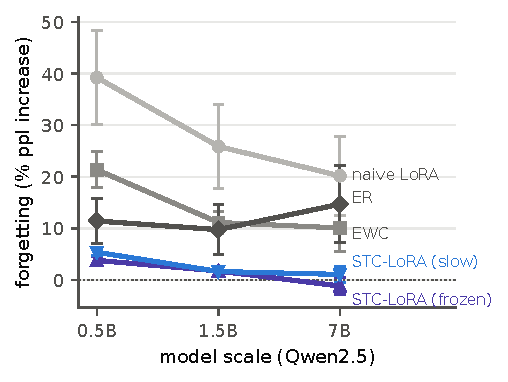
\includegraphics[width=.48\linewidth]{figs/scaling.pdf}\hfill
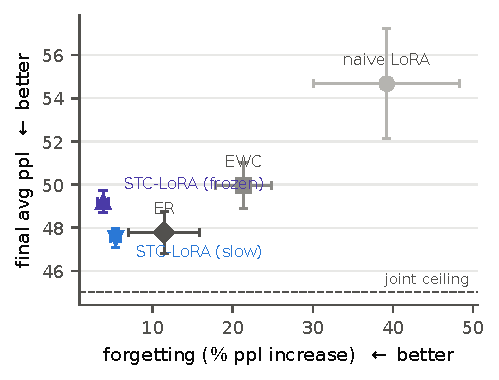
\includegraphics[width=.48\linewidth]{figs/pareto.pdf}
\caption{\textbf{Left:} forgetting vs.\ scale (mean $\pm$ std over 4 seed$\times$order replicates). Scale alone does not solve forgetting for the baselines; \stc{} sits at ${\approx}0$ throughout. \textbf{Right:} stability--plasticity at 0.5B; \stc{} variants occupy the Pareto corner nearest the joint ceiling.}
\label{fig:scaling}
\end{figure}

\begin{figure}[t]
\centering
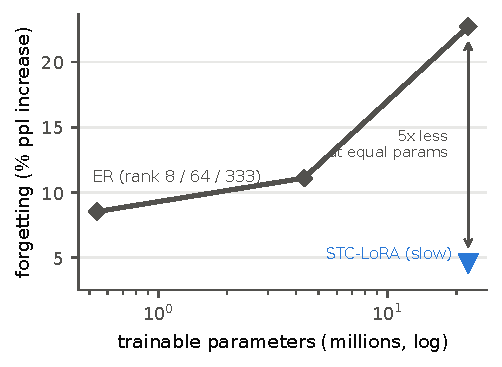
\includegraphics[width=.6\linewidth]{figs/capacity.pdf}
\caption{Capacity-matched control: ER's forgetting \emph{grows} with adapter size; at parameter parity (22.5M) \stc{} forgets $5\times$ less. The advantage is the mechanism, not the parameters.}
\label{fig:capacity}
\end{figure}

Table~\ref{tab:scale} and Figure~\ref{fig:scaling}: the ordering is identical at every scale and on both families. Two observations. (i) \emph{Scale does not solve forgetting}: at 7B, naive still forgets $+20\%$ and ER $+15\%$, while \stc{} sits at ${\approx}0\%$ --- frequently \emph{negative} (learning later domains improves earlier ones). (ii) On the more forgetting-prone Llama base (naive $+41\%$), the protection is proportionally larger; on that family ER retains a small final-perplexity edge (30.3 vs.\ 31.9), so the family-general claim is about forgetting and its order-robustness, with quality competitive. At 1.5B and 7B, the slow-store variant wins \emph{both} axes (e.g.\ 1.5B: forgetting $1.6$ vs.\ ER's $9.7\%$; ppl 27.1 vs.\ 28.1 against a 26.4 ceiling).

\subsection{Capacity-matched control}
Figure~\ref{fig:capacity}: ER's forgetting \emph{worsens monotonically} as its adapter grows (rank 8/64/333 $\Rightarrow$ $8.5/11.1/22.7\%$): extra capacity is spent overwriting faster. At parameter parity with \stc{}'s permanent store (22.5M), \stc{} forgets $4.6\%$ vs.\ ER's $22.7\%$ --- $5\times$ less at equal size, with better perplexity (47.4 vs.\ 50.6). The advantage is the structured two-timescale mechanism, not parameters. (Measured at the 200-chunk configuration.)

\subsection{Downstream forgetting: capability, not calibration}\label{sec:downstream}
\begin{table}[t]
\centering\small
\caption{Task-level forgetting (0.5B, seed 0): drop after the stream moves past the news domain. Zero-shot column has binomial noise ${\sim}\pm4$ points ($n{=}150$).}
\label{tab:downstream}
\begin{tabular}{lcc}
\toprule
method & news token-acc drop $\downarrow$ & AG News zero-shot drop $\downarrow$ \\
\midrule
naive & $+14.0\%$ & $+1.6\%$ \\
EWC & $+9.3\%$ & $+13.2\%$ \\
ER & $+5.6\%$ & $+11.8\%$ \\
\stc{} (frozen) & $+3.4\%$ & $\best{-6.5\%}$ \\
\stc{} (slow) & $\best{+2.8\%}$ & $+8.7\%$ \\
\bottomrule
\end{tabular}
\end{table}

Because perplexity-based forgetting could in principle reflect calibration drift, we measure top-1 next-token accuracy and AG~News zero-shot classification (label-word log-likelihood) on the identical protocol. Learning the news domain first \emph{improves} zero-shot accuracy over the frozen base ($0.35\rightarrow0.42$--$0.51$); the subsequent drop is genuine capability forgetting. Token-accuracy forgetting (Table~\ref{tab:downstream}) reproduces the perplexity ordering exactly; \stc{} loses $5\times$ less capability than naive, and the frozen-store variant shows \emph{positive} transfer on the real task.

\subsection{The gate buys allocation, not raw stability}
The surprise gate must beat a matched non-adaptive ablation. Three arms, identical seed/data, differing only in $m$: the gate; $m\equiv0.5$ (the gate's neutral output --- matched average plasticity, no adaptivity, consolidation intact); $m\equiv1$ (maximal plasticity, capture every chunk):
\begin{center}\small
\begin{tabular}{lccc}
\toprule
arm & forgetting \% & final ppl & captures \\
\midrule
gated & $\best{+4.5}$ & $\best{47.3}$ & 462 \\
$m\equiv0.5$ & $+4.5$ & $49.0$ & 480 \\
$m\equiv1.0$ & $+5.0$ & $47.7$ & 1079 \\
\bottomrule
\end{tabular}
\end{center}
Versus matched-average plasticity the gate ties on forgetting but improves final perplexity by $1.7$: adaptivity spends the same total plasticity where surprise indicates it matters --- an \emph{allocation} mechanism. Versus always-maximal it wins both axes while consolidating $2.3\times$ less often.

\subsection{Component analysis and cost}
Consolidation alone (no replay) already halves ER's forgetting; the slow-plastic store is a clean stability--plasticity knob ($\rho{:}\,0\rightarrow0.05$ recovers ER-level fluency at a small forgetting cost; $\rho{=}0.1$ shows diminishing returns). Wall-clock per stream at 1.5B (A6000): naive 75s, EWC 91s, ER 128s, \stc{} 128--134s --- \stc{} costs the same as ER at matched budget; decay and capture are negligible ($O(r\,d)$ and a rank-$r$ product).

\section{Limitations}
(1) \emph{Recognition vs.\ recall}: gradient consolidation reliably improves distributional familiarity (perplexity, token accuracy) but does not by itself make individual facts retrievable in QA; targeted editing \citep{meng2022locating} is the complementary tool. (2) \emph{Scope}: three English registers; downstream metrics at 0.5B/seed-0 only; two model families. (3) \emph{Adversarial streams}: the self-loss gate is unexamined under data poisoning, where surprise-seeking could be exploited. (4) \emph{Memory}: the dense permanent store is $O(d_o d_i)$ per layer; a low-rank store is future work (our capacity-fair control suggests the mechanism, not the dense capacity, carries the benefit).

\section{Conclusion}
\stc{} turns a frozen LM into an online continual learner by giving its adapter two timescales and a significance gate: transient changes decay unless captured into a protected, slowly-refining permanent store. Across three scales and two families it cuts forgetting to single digits --- near zero at 7B --- at replay-matched cost, with the strongest order-robustness among all methods tested, and the protection is visible in task capability, not just perplexity.

\paragraph{Reproducibility.} Code, benchmark harness, and the JSON artifacts behind every table and figure: \url{https://github.com/kfchai/stc_lora}. % NOTE: anonymize this URL for double-blind submission.

\bibliographystyle{unsrtnat}
\bibliography{refs}

\appendix
\section{Reservoir uniformity is load-bearing}
With a recency-biased buffer, consolidation replay \emph{hurt} ($+23.4\%$ forgetting vs.\ $+16.7\%$ without replay); replacing it with uniform reservoir sampling \citep{vitter1985random} made the same mechanism the best method ($+4.3\%$). In boundary-free online CL, the buffer must be temporally uniform; surprise should weight \emph{replay strength}, not buffer \emph{membership}.

\section{Hyperparameters}
Rank $r{=}8$, $\alpha{=}16$, targets = attention q/v projections; $\eta_0{=}5{\times}10^{-2}$; decay $\lambda{=}0.08$; capture threshold $\tau{=}0.6$, capture fraction $0.6$; reservoir 40 chunks, replay every 100 steps $\times$ 2 rounds, sleep boost $1.6$; $\rho{=}0.05$. EWC $\lambda{=}100$ (swept over $\{10,100,10^3,5{\times}10^4\}$); ER replay ratio matched to \stc{} consolidation compute ($\approx$480 extra steps). bf16 at 1.5B/7B, fp32 at 0.5B.
\end{document}
